

\chapter{Functions}\label{chapter:functions}


In this chapter we explore general functions from tensors into other tensors.
While not quite as elegant as linear functions, they are important for many applications, such as non-linearities in neural networks.
The main goal is to make the vector chain rule intuitive and easy to apply, but we also cover Taylor series, determinants and other topics.

Standard notation for function over vectors can be quite ambiguous when the function broadcasts over some dimensions.
If $x\in\R^n$ is a vector, it's not clear whether $f(x)$ applies to each element of $x$ independently or if it's a function of the whole vector.
With tensor diagrams, we make this distinction clear by explicitly showing the edges of $x$ that go into $f$, and which don't.
We use the notation 
%If the result of $f(x)$ is itself a vector $\in\R^m$, we can write
\tikz[baseline=-.25em, inner sep=2pt]{
   \draw[->] (.5,0) node[right]{$x$} -- node[above, font=\tiny]{$n$} (0,0) node(f)[left]{$f$};
   \draw (f) -- ++(-.5,0) node[midway, above, font=\tiny] {$m$};
}
when $f$ is a function from $\R^n$ to $\R^m$.
If $f$ is element-wise, we write
$(\tikz[baseline=-.25em, inner sep=2pt]{
   \draw[->, densely dotted] (.3,0) node[right](x){$x$} -- (0,0) node(f)[left]{$f$};
   \draw (x) -- ++(.5,0) node[midway, above, font=\tiny] {$n$};
}) \in \R^n$.
We always assume that the function (arrow) edges are contracted before normal edges.
If we want something else, like $f(Mx)$, we can use brackets:
\tikz[baseline=(f.base), inner xsep=2pt, inner ysep=0pt]{
   \node (f) at (0,0) {$f$};
   \draw (f) -- ++(-.5,0);
   \node (group) at (1.5,0) {$(
      \tikz {
         \node (M) at (0.5,0) {$M$};%
         \draw (0,0) -- (M) -- ++(.5,0) node[right]{$x$};%
      }%
      )$
   };
   \draw[->] (group) -- (f);
}.
It may be helpful with some more examples:
%In the examples below, $x\in \R^n$:
\vspace{-1.5em}
\begin{center}
\begingroup
\renewcommand{\arraystretch}{2.5}
\begin{tabular}[h]{cccc}
   $f : \mathbb R^n \to \mathbb R$
   & $f(x) \in \mathbb R$
   & \tikz[baseline=-.25em]{\draw[->] (.5,0) node[right]{$x$} -- node[above, font=\tiny]{$n$} (0,0) node[left]{$f$}}
   & (Scalar function)
   \\
   $g : \mathbb R^n \to \mathbb R^m$
   & $g(x) \in \mathbb R^m$
   & \tikz[baseline=(x.base)]{
      \node (x) at (0,0) {$x$};
      \node (g) at (-.75,0) {$g$};
      \draw[->] (x) -- (g) node[midway, above, font=\tiny] {$n$};
      \draw (g) -- ++(-.5,0) node[midway, above, font=\tiny] {$m$};
   }
   & (Vector function)
   \\
   $h : \mathbb R \to \mathbb R$
   & $h(x) \in \mathbb R^n$
   & \tikz[baseline=(x.base)]{
      \node (x) at (0,0) {$x$};
      \node (h) at (-.75,0) {$h$};
      \draw[->, densely dotted] (x) -- (h);
      \draw (x) -- ++(.5,0) node[right, font=\tiny] {$n$};
   }
   & (Element-wise function)
   \\
   \makecell[c]{$u : \mathbb{R}^n \to \mathbb{R}^m$ \\ $v \in \mathbb{R}^m$}
   & $v^T u(x) \in \mathbb R$
   & \tikz[baseline=(x.base)]{
      \node (x) at (0,0) {$x$};
      \node (v) at (-.75,0) {$v$};
      \node (u) at (-1.5,0) {$u$};
      \draw[->] (x) -- (v) node[midway, above, font=\tiny] {$n$};
      \draw (v) -- (u) node[midway, above, font=\tiny] {$m$};
   }
   & (Vector times vector function)
   \\
   \makecell[c]{$A : \mathbb R^n \to \mathbb R^{m\times n},$\\$v \in \mathbb R^n$}
   & $A(x)v \in \mathbb R^m$
   & 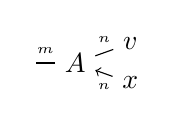
\begin{tikzpicture}[baseline=(A.base)]
      \node (A) at (0,0) {$A$};
      \draw (A) -- ++(-.5,0) node[midway, above, font=\tiny] {$m$};
      \node (x) at (.7,-.25) {$x$};
      \draw[->] (x) -- (A) node[midway, below, font=\tiny] {$n$};
      \node (v) at (.7,.25) {$v$};
      \draw (v) -- (A) node[midway, above, font=\tiny] {$n$};
   \end{tikzpicture}
   & (Vector times matrix function)
   \\
   \makecell[c]{$A : \mathbb R^{n\times m} \to \mathbb R,$\\$X \in \mathbb R^{n\times m}$}
   & $A(X) \in \R$
   & 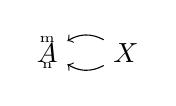
\begin{tikzpicture}[baseline=-.25em]
      \node (A) at (0,0) {$A$};
      \node (X) at (1,0) {$X$};
      \draw[->] (X) edge[bend left] (A) node[midway, above, font=\tiny] {m};
      \draw[->] (X) edge[bend right] (A) node[midway, below, font=\tiny] {n};
   \end{tikzpicture}
   & (Matrix function)
   \\
   \makecell[c]{$f : \mathbb R^d \to \mathbb R,$\\$X \in \mathbb R^{b\times d}$}
   & $f(X) \in \mathbb R^b$
   & 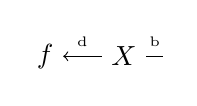
\begin{tikzpicture}[baseline=-.25em]
      \node (f) at (0,0) {$f$};
      \node (X) at (1,0) {$X$};
      \draw[->] (X) -- (f) node[midway, above, font=\tiny] {d};
      \draw (X) --  ++(.5,0) node[midway, above, font=\tiny] {b};
   \end{tikzpicture}
   & (Batch function application)
   \\
   \makecell[c]{
      $f : \mathbb R^n\times \R^m \to \R^d$
      ,\\$u \in \mathbb R^{b\times n}
      , v \in \R^{b\times m}$
   }
   & $f(u, v) \in \R^{b \times d}$
   & 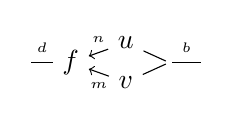
\begin{tikzpicture}[baseline=-.25em]
      \node (f) at (0,0) {$f$};
      \draw (f) -- ++(-.5,0) node[midway, above, font=\tiny] {$d$};
      \node (u) at (.7,.25) {$u$};
      \draw[->] (u) -- (f) node[midway, above, font=\tiny] {$n$};
      \node (v) at (.7,-.25) {$v$};
      \draw[->] (v) -- (f) node[midway, below, font=\tiny] {$m$};
      \node[inner sep=1pt] (d) at (1.25,0) {$\sbullet$};
      \draw (u) -- (d);
      \draw (v) -- (d);
      \draw (d) -- ++(.4,0) node[midway, above, font=\tiny] {$b$};
   \end{tikzpicture}
   & (Two inputs, batched)
\end{tabular}
\endgroup
\end{center}

To make it more concrete, let's consider some well known functions:
Let $\mathrm{pow}(n) : \mathbb R \to \mathbb R$ be the element-wise power function, and $\mathrm{exp} : \mathbb R \to \mathbb R$ be the element-wise exponential function.
Then we can write $\mathrm{softmax}:\mathbb R^d \to \mathbb R^d$ as the tensor diagram:
\[
   \mathrm{softmax}(x) =
   \begin{tikzpicture}[baseline=-.25em]
      \node (ex) at (0,0) {$\{\mathrm{exp} \quad x\}$};
      \node[right=1em of ex] (p) {$\{\mathrm{pow}(-1) \quad \{\mathrm{exp} \quad x\}\quad \sbullet\,\}$};
      \draw ($(p.east)+(-1.1,.15)$) edge[out=90, in=90, looseness=1] ($(p.east)+(-.4,.15)$);
      \draw ($(ex) + (.5, .15)$) -- ++(.1,.2);
   \end{tikzpicture}
   .
\]


\begin{align*}
   \mathrm{pow}^{-1} x
\end{align*}

In the diagrams above the “curved” or “straight” edges indicate the flow of indices. When an edge is left free, it represents an output index of the function; a connected edge denotes a contracted (summed over) index. For example, applying a scalar function $f$ to a vector $x$ is written as $\{f\leftarrow x\}$, meaning the $n$-dimensional $x$ flows into $f$ and the result, being a scalar, has no free edges.


As an example of a more complicated function, let $\exp : \mathbb R \to \mathbb R$ be the element-wise exponential function,
and $\mathrm{pow}^{-1} : \mathbb R \to \mathbb R$ be the element-wise inverse power function.
Then we can write $\mathrm{softmax}:\mathbb R^d \to \mathbb R^d$ as the tensor diagram:
\[
   \mathrm{softmax}(x) =
   \begin{tikzpicture}[baseline=-.25em]
      \node (ex) at (0,0) {$\{\mathrm{exp} \quad x\}$};
      \node[right=1em of ex] (p) {$\{\mathrm{pow}^{-1} \quad \{\mathrm{exp} \quad x\}\quad \sbullet\,\}$};
      \draw ($(p.east)+(-1.1,.15)$) edge[out=90, in=90, looseness=1] ($(p.east)+(-.4,.15)$);
      \draw ($(ex) + (.5, .15)$) -- ++(.1,.2);
   \end{tikzpicture}
   .
\]
Note in particular how
\begin{tikzpicture}[baseline=-.25em]
   \node (p) {$\{\mathrm{exp} \quad x\}\quad \sbullet$};
   \path ($(p.east)+(-.9,.15)$) edge [out=90, in=90, looseness=1] ($(p.east)+(-.2,.15)$);
\end{tikzpicture}
is the diagram way of writing $\sum_i \exp(x_i)$.
Alternatively we could have used a function $\mathrm{sum} : \mathbb R^n \to \mathbb R$, but the more we can express in terms of tensor diagrams, the more we can use the powerful tensor diagram calculus.



Stuff about analytical matrix functions.
Such as Exponential Matrix Function.
I'd rather talk about my general function notation.
And maybe about taylor series?


\newpage
\section{The Chain Rule}
Sometimes the objective is to find the derivative of a matrix which is a function of another matrix.

E.g. $f : \R^n -> \R^n$

Standard chain rule.
Here we let $f\in\mathbb R^d\to \mathbb R$ be a scalar function, and $v\in\mathbb R^d\to \mathbb R^d$ be a vector function as used in backprop.

Visualization of the Chain Rule: $J_{f\circ v}(x) = \nabla_{\!f}(v(x)) J_v(x)$.

\[
   \begin{tikzpicture}[baseline=-.25em, inner sep=1pt]
      \node (n1) {$(\quad\{$};
      \node[right=.5em of n1] (n2) {$f$};
      \node[right=.5em of n2] (n3) {$\{$};
      \node[right=0em of n3] (n4) {$v$};
      \node[right=1em of n4] (n5) {$x$};
      \node[right=0em of n5] (n6) {$\}\}\quad)$};
      \draw (n4) edge[out=90, in=90, looseness=1, ->] (n2);
      \draw (n5) edge[->] (n4);
      \draw[d] (n6.east) -- ++(.2,.2);
   \end{tikzpicture}
   =
   \begin{tikzpicture}[baseline=-.25em, inner sep=1pt]
      \node (n1) {$\{$};
      \node[right=.5em of n1] (n2) {$f$};
      \node[right=.5em of n2] (n3) {$\{$};
      \node[right=0em of n3] (n4) {$v$};
      \node[right=1em of n4] (n5) {$x$};
      \node[right=0em of n5] (n6) {$\}\}$};
      \node[right=1em of n6] (n7) {$\{$};
      \node[right=0em of n7] (n8) {$v$};
      \node[right=1em of n8] (n9) {$x$};
      \node[right=0em of n9] (n10) {$\}$};
      \draw (n4) edge[out=90, in=90, looseness=1, ->] (n2);
      \draw (n5) edge[->] (n4);
      \draw (n9) edge[->] (n8);
      \draw[d1] (n2) edge[out=-30, in=-120, looseness=1] (n8);
      \draw[d1] (n8) -- ++(.3,.3);
   \end{tikzpicture}
\]

\subsection{The Chain Rule}
Let $f\in\mathbb R^d\to \mathbb R$ be a scalar function, and $v\in\mathbb R^d\to \mathbb R^d$ be a vector function, as used in backprop.
Then we can write the chain rule as:
\[
   \begin{tikzpicture}[baseline=-1em, inner sep=1pt]
      \node (n0) {$f$};
      \node[below=1em of n0] (n1) {$v$};
      \node[below=1em of n1] (n2) {$x$};
      \draw[->] (n2) -- (n1);
      \draw[->] (n1) -- (n0);
      \drawellipse{0}{-.55}{.5}{1}{180/4}
   \end{tikzpicture}
   =
   \hspace{.5em}
   \begin{tikzpicture}[baseline=-1em, inner sep=1pt]
      \node[dn] (n0) {$f$};
      \node[below=1em of n0] (n1) {$v$};
      \node[below=1em of n1] (n2) {$x$};
      \node[right=1em of n0, dn] (n3) {$v$};
      \node[below=1em of n3] (n4) {$x$};
      \draw[->] (n2) -- (n1);
      \draw[->] (n1) -- (n0);
      \draw[->] (n4) -- (n3);
      \draw[d0] (n0) -- (n3);
      \draw[d0] (n3) -- ++(.5,0);
   \end{tikzpicture}
\]
Using standard notation:
$J_{f\circ v}(x) = \nabla_{\!f}(v(x)) J_v(x)$.

\vspace{1em}

The second derivative, (or Hessian Chain rule):
\[
   \begin{tikzpicture}[baseline=-1em, inner sep=1pt]
      \node (n0) {$f$};
      \node[below=1em of n0] (n1) {$v$};
      \node[below=1em of n1] (n2) {$x$};
      \draw[->] (n2) -- (n1);
      \draw[->] (n1) -- (n0);
      \drawellipse{0}{-.55}{.5}{1}{180/4}
      \drawellipse{0}{-.55}{.7}{1.2}{180/4}
   \end{tikzpicture}
   =
   \hspace{.5em}
   \begin{tikzpicture}[baseline=-1em, inner sep=1pt]
      \node[dn] (n0) {$f$};
      \node[below=1em of n0] (n1) {$v$};
      \node[below=1em of n1] (n2) {$x$};
      \node[right=1em of n0, dn] (n3) {$v$};
      \node[below=1em of n3] (n4) {$x$};
      \draw[->] (n2) -- (n1);
      \draw[->] (n1) -- (n0);
      \draw[->] (n4) -- (n3);
      \draw[d0] (n0) -- (n3);
      \draw[d0] (n3) -- ++(.5,0);
      \drawellipse{.4}{-.55}{1}{1.2}{180/4}
   \end{tikzpicture}
   =
   \hspace{.5em}
   \begin{tikzpicture}[baseline=-1em, inner sep=1pt]
      \node[dn] (n0) {$f$};
      \node[below=1em of n0] (n1) {$v$};
      \node[below=1em of n1] (n2) {$x$};
      \node[right=1.5em of n0, dn] (n3) {$v$};
      \node[below=1em of n3] (n4) {$x$};
      \draw[->] (n2) -- (n1);
      \draw[->] (n1) -- (n0);
      \draw[->] (n4) -- (n3);
      \draw[d0] (n0) -- (n3);
      \draw[d0] (n3) -- ++(.5,0);
      \drawellipse{0}{-.55}{.5}{1.2}{180/4}
   \end{tikzpicture}
   +
   \hspace{.5em}
   \begin{tikzpicture}[baseline=-1em, inner sep=1pt]
      \node[dn] (n0) {$f$};
      \node[below=1em of n0] (n1) {$v$};
      \node[below=1em of n1] (n2) {$x$};
      \node[right=1.5em of n0, dn] (n3) {$v$};
      \node[below=1em of n3] (n4) {$x$};
      \draw[->] (n2) -- (n1);
      \draw[->] (n1) -- (n0);
      \draw[->] (n4) -- (n3);
      \draw[d0] (n0) -- (n3);
      \draw[d0] (n3) -- ++(.5,0);
      \drawellipse{1}{-.25}{.5}{.7}{180/4}
   \end{tikzpicture}
   =
   \hspace{.5em}
   \begin{tikzpicture}[baseline=-1em, inner sep=1pt]
      \node[ddn] (n0) {$f$};
      \node[below=1em of n0] (n1) {$v$};
      \node[below=1em of n1] (n2) {$x$};
      \node[right=1em of n0, yshift=-1em, dn] (n3) {$v$};
      \node[below=1em of n3] (n4) {$x$};
      \node[right=1.5em of n3, yshift=1em, dn] (n5) {$v$};
      \node[below=1em of n5] (n6) {$x$};
      \draw[->] (n2) -- (n1);
      \draw[->] (n1) -- (n0);
      \draw[->] (n4) -- (n3);
      \draw[->] (n6) -- (n5);
      \draw[d0] (n0) -- (n3);
      \draw[d0] (n0) -- (n5);
      \draw[d0] (n3) -- ++(.5,0);
      \draw[d0] (n5) -- ++(.5,0);
   \end{tikzpicture}
   +
   \hspace{.5em}
   \begin{tikzpicture}[baseline=-1em, inner sep=1pt]
      \node[dn] (n0) {$f$};
      \node[below=1em of n0] (n1) {$v$};
      \node[below=1em of n1] (n2) {$x$};
      \node[right=1.5em of n0, ddn] (n3) {$v$};
      \node[below=1em of n3] (n4) {$x$};
      \draw[->] (n2) -- (n1);
      \draw[->] (n1) -- (n0);
      \draw[->] (n4) -- (n3);
      \draw[d0] (n0) -- (n3);
      \draw[d0] (n3) -- ++(.5,0);
      \draw[d0] ($(n3)+(.166,.15)$) -- ++(.4,0);
   \end{tikzpicture}
\]
Using standard notation:
\(
H_{f\circ v}(x) = Dv(x)^T \cdot D^2f(v(x)) \cdot Dv(x) + \sum_{k=1}^d \frac{\partial f}{\partial u_k}(v(x)) \frac{\partial^2 v_k}{\partial x \partial x^T}(x).
\)


\begin{align*}
\hspace{-2em}
   \frac{\partial A(x)x}{\partial x}
   &= (x^T \otimes I) \frac{\partial}{\partial x}  \mathrm{vec}[A(x)] + A(x)
   &
   \begin{tikzpicture}[baseline=-.25em, inner sep=1pt]
      \node (n0) at (0,0) {$($};
      \node[right=.5em of n0] (x0) {$x$};
      \node[right=.5em of x0] (n2) {$\{$};
      \node[right=.5em of n2] (A) {$A$};
      \node[right=1em of A] (x1) {$x$};
      \node[right=.5em of x1] (n5) {$\})$};
      \draw[->] (x1) -- (A);
      \draw (x0) edge[out=90, in=90, looseness=1] (A);
      \draw[d] (n5.east) -- ++(.2,.2);
   \end{tikzpicture}
   &=
   \begin{tikzpicture}[baseline=-.25em, inner sep=1pt]
      \node (x0) {$x$};
      \node [right=.5em of x0] (n2) {$(\{$};
      \node [right=.5em of n2] (A) {$A$};
      \node [right=1em of A] (x1) {$x$};
      \node [right=.5em of x1] (n5) {$\})$};
      \draw[->] (x1) -- (A);
      \draw (x0) edge[out=90, in=90, looseness=1] (A);
      \draw[d] (n5.east) -- ++(.2,.2);
   \end{tikzpicture}
 +
   \begin{tikzpicture}[baseline=-.25em, inner sep=1pt]
      \node (n0) at (0,0) {$($};
      \node [right=.5em of n0] (x0) {$x$};
      \node [right=.5em of x0] (n1) {$)$};
      \node [right=.5em of n1] (n2) {$\{$};
      \node [right=.5em of n2] (A) {$A$};
      \node [right=1em of A] (x1) {$x$};
      \node [right=.5em of x1] (n5) {$\}$};
      \draw[->] (x1) -- (A);
      \draw (x0) edge[out=90, in=90, looseness=1] (A);
      \draw[d] (n1.east) -- ++(.2,.2);
   \end{tikzpicture}
 \\&&&=
   \begin{tikzpicture}[baseline=-.25em, inner sep=1pt]
      \node (x0) {$x$};
      \node [right=.5em of x0] (n2) {$\{$};
      \node [right=.5em of n2] (A) {$A$};
      \node [right=1em of A] (x1) {$x$};
      \node [right=.5em of x1] (n5) {$\}$};
      \draw[->] (x1) -- (A);
      \draw (x0) edge[out=90, in=90, looseness=1] (A);
      \draw[d] ($(A.east)+(.1,.1)$) -- ++(.3,.2);
   \end{tikzpicture}
 +
   \begin{tikzpicture}[baseline=-.25em, inner sep=1pt]
      \node (n2) {$\{$};
      \node [right=.5em of n2] (A) {$A$};
      \node [right=1em of A] (x1) {$x$};
      \node [right=.5em of x1] (n5) {$\}$};
      \draw[->] (x1) -- (A);
      \draw (A) -- ++(.4,.3);
   \end{tikzpicture}
\end{align*}

\[
   \begin{tikzpicture}[baseline=-1em, inner sep=1pt]
      \node (n0) {$A$};
      \node[below=1em of n0] (n1) {$x$};
      \node[right=1em of n0] (n2) {$x$};
      \draw[->] (n1) -- (n0);
      \draw (n2) -- (n0);
      \drawellipse{.25}{-.25}{.7}{.7}{180/4}
      \draw (n0) -- ++(-.5,0);
   \end{tikzpicture}
   =
   \hspace{.5em}
   \begin{tikzpicture}[baseline=-1em, inner sep=1pt]
      \node (n0) {$A$};
      \node[below=1em of n0] (n1) {$x$};
      \node[right=1em of n0] (n3) {$x$};
      \draw[->] (n1) -- (n0);
      \draw (n0) -- (n3);
      \drawellipse{0}{-.25}{.4}{.7}{180/4}
      \draw (n0) -- ++(-.5,0);
   \end{tikzpicture}
   +
   \hspace{.5em}
   \begin{tikzpicture}[baseline=-1em, inner sep=1pt]
      \node (n0) {$A$};
      \node[below=1em of n0] (n1) {$x$};
      \node[right=.75em of n0] (n3) {$x$};
      \draw[->] (n1) -- (n0);
      \draw (n0) -- (n3);
      \draw (n0) -- ++(-.5,0);
      \drawellipse{.575}{0}{.25}{.25}{180/4}
   \end{tikzpicture}
   =
   \hspace{.5em}
   \begin{tikzpicture}[baseline=-1em, inner sep=1pt]
      \node[dn] (n0) {$A$};
      \node[below=1em of n0] (n1) {$x$};
      \node[right=.75em of n0] (n3) {$x$};
      \draw[->] (n1) -- (n0);
      \draw (n0) -- (n3);
      \draw[d0] (n0) -- ++(.4,.4);
      \draw (n0) -- ++(-.5,0);
   \end{tikzpicture}
   +
   \hspace{.5em}
   \begin{tikzpicture}[baseline=-1em, inner sep=1pt]
      \node (n0) {$A$};
      \node[below=1em of n0] (n1) {$x$};
      \draw[->] (n1) -- (n0);
      \draw (n0) -- ++(.5,0);
      \draw (n0) -- ++(-.5,0);
   \end{tikzpicture}
\]


are common. All pixel-adaptive filters like non-local means, bilateral, etc, and the so-called attention mechanism in transformers can be written this way

Gradient of this f(x) is important \& has a form worth remembering…


\subsubsection{Trace identity}
Assume F(X) to be a differentiable function of each of the elements of X. It
then holds that
\[\frac{d \mathrm{Tr}(F(x))}{dX} = f(X)^T,\]
where $f(\cdot)$ is the scalar derivative of $F(\cdot)$.

TODO: To show this with tensor diagrams, we first need to introduce our notation for functions.

For example
$$
\frac{\partial \operatorname{Tr}(\sin (\mathbf{X}))}{\partial \mathbf{X}}=\cos (\mathbf{X})^T
$$
% Many more examples here: https://mbustamanter.github.io/ssg-blog/matder1/


\subsubsection{Pseudo-linear form}
Maybe this should just be an example in a table?

Derivation of Peyman Milanfar's gradient
\begin{align*}
\mathrm{d}[\mathbf{f}(\mathbf{x})] & =\mathrm{d}[\mathbf{A}(\mathbf{x}) \mathbf{x}] \\
& =\mathrm{d}[\mathbf{A}(\mathbf{x})] \mathbf{x}+\mathbf{A}(\mathbf{x}) \mathrm{d} \mathbf{x} \\
& =\operatorname{vec}\{\mathrm{d}[\mathbf{A}(\mathbf{x})] \mathbf{x}\}+\mathbf{A}(\mathbf{x}) \mathrm{d} \mathbf{x} \\
& =\operatorname{vec}\{\mathbf{I} \mathrm{d}[\mathbf{A}(\mathbf{x})] \mathbf{x}\}+\mathbf{A}(\mathbf{x}) \mathrm{d} \mathbf{x} \\
& =\left(\mathbf{x}^T \otimes \mathbf{I}\right) \operatorname{vec}\{\mathrm{d}[\mathbf{A}(\mathbf{x})]\}+\mathbf{A}(\mathbf{x}) \mathrm{d} \mathbf{x} \\
& =\left(\mathbf{x}^T \otimes \mathbf{I}\right) \mathrm{D} \operatorname{vec}[\mathbf{A}(\mathbf{x})] \mathrm{d} \mathbf{x}+\mathbf{A}(\mathbf{x}) \mathrm{d} \mathbf{x} \\
& =\left[\left(\mathbf{x}^T \otimes \mathbf{I}\right) \mathrm{D} \operatorname{vec}[\mathbf{A}(\mathbf{x})]+\mathbf{A}(\mathbf{x})\right] \mathrm{d} \mathbf{x}
\end{align*}

\subsection{Taylor}
For an n-times differentiable function $v: \R^d\to\R^d$ we can write the Taylor expansion:
\begin{align*}
    v(x + \eps)
    &\approx
    v(x)
    + \left[\frac{\partial}{\partial x} v(x)\right]\eps
    + \frac{1}{2}\left[\frac{\partial}{\partial x}\left[\frac{\partial}{\partial x} v(x)\right]\eps\right]\eps
    + \frac{1}{6}\left[\frac{\partial}{\partial x}\left[\frac{\partial}{\partial x} \left[\frac{\partial}{\partial x} v(x)\right]\eps\right]\eps\right]\eps
    + \dots
    \\
    &=
    v(x)
    + \left[\frac{\partial}{\partial x} v(x)\right]\eps
    +
    \frac{1}{2}
    (I \otimes \eps)
    \left[\frac{\partial\mathrm{vec}}{\partial x}\left[\frac{\partial v(x)}{\partial x} \right]\right]\eps
    + \frac{1}{6}
    (I \otimes \eps \otimes \eps)
    \left[\frac{\partial\mathrm{vec}}{\partial x}\left[\frac{\partial\mathrm{vec}}{\partial x} \left[\frac{\partial v(x)}{\partial x} \right]\right]\right]\eps
    + \dots
\end{align*}
Or with indices:
\begin{align*}
    v_i(x + \eps)
    &\approx
    v_i(x)
    + \sum_j \frac{\partial v_i(x)}{\partial x_j} \eps_j
    + \frac12 \sum_{j,k} \frac{\partial^2 v_i(x)}{\partial x_j\partial x_k} \eps_j \eps_k
   + \frac16 \sum_{j,k,\ell} \frac{\partial^3 v_i(x)}{\partial x_j\partial x_k\partial x_\ell} \eps_j \eps_k \eps_\ell
\end{align*}
Or diagrams:
\[
   \begin{tikzpicture}[baseline=-1em, inner sep=1pt]
      \node (n0) {$v$};
      \node[below=1em of n0] (n1) {$(x+\eps)$};
      \draw[->] (n1) -- (n0);
      \draw (n0) -- ++(.5,0);
   \end{tikzpicture}
   \approx
   \begin{tikzpicture}[baseline=-1em, inner sep=1pt]
      \node (n0) {$v$};
      \node[below=1em of n0] (n1) {$x$};
      \draw[->] (n1) -- (n0);
      \draw (n0) -- ++(.5,0);
   \end{tikzpicture}
   +
   \begin{tikzpicture}[baseline=-1em, inner sep=1pt]
      \node[dn] (n0) {$v$};
      \node[below=1em of n0] (n1) {$x$};
      \node[left=1em of n0] (n2) {$\eps$};
      \draw[->] (n1) -- (n0);
      \draw[d0] (n0) -- (n2);
      \draw (n0) -- ++(.5,0);
   \end{tikzpicture}
   +\frac12
   %\hspace{.5em}
   \begin{tikzpicture}[baseline=-1em, inner sep=1pt]
      \node[ddn] (n0) {$v$};
      \node[below=1em of n0] (n1) {$x$};
      \node[left=1em of n0] (n2) {$\eps$};
      \node[left=.75em of n0, yshift=-1em] (n3) {$\eps$};
      \draw[->] (n1) -- (n0);
      \draw[d0] (n0) -- (n2);
      \draw[d0] (n0) -- (n3);
      \draw (n0) -- ++(.5,0);
   \end{tikzpicture}
   +
   \frac16
   %\hspace{.5em}
   \begin{tikzpicture}[baseline=-1em, inner sep=1pt]
      \node[dddn] (n0) {$v$};
      \node[below=1em of n0] (n1) {$x$};
      \node[left=1em of n0] (n2) {$\eps$};
      \node[left=.75em of n0, yshift=-1em] (n3) {$\eps$};
      \node[left=.75em of n0, yshift=1em] (n4) {$\eps$};
      \draw[->] (n1) -- (n0);
      \draw[d0] (n0) -- (n2);
      \draw[d0] (n0) -- (n3);
      \draw[d0] (n0) -- (n4);
      \draw (n0) -- ++(.5,0);
   \end{tikzpicture}
   +
   \dots
\]

TODO: Examples based on idempotent matrices etc.



\section{Exercises}
\begin{exercise}
   Draw the tensor diagram for a function $f:\mathbb{R}^n\to\mathbb{R}$ that applies an element-wise nonlinearity (for instance, $\exp$) followed by a summation over the components. Verify that the diagram corresponds to the conventional formula for the softmax denominator.
\end{exercise}

\begin{exercise}
   Represent the composition of two functions 
   \[
      f:\mathbb{R}^m\to\mathbb{R} \quad \text{and} \quad v:\mathbb{R}^n\to\mathbb{R}^m,
   \]
   using tensor diagrams. Then, using the diagrammatic chain rule, derive the expression for the derivative of $f\circ v$ with respect to $x\in\mathbb{R}^n$.
\end{exercise}

\begin{exercise}
   For a matrix function $A(x)$ that depends on a vector $x$, use tensor diagrams to illustrate the derivative 
   \[
      \frac{\partial}{\partial x}[A(x)x],
   \]
   and explain how the product rule is implemented in the diagram.
\end{exercise}

\begin{exercise}
   % Source: Adapted from StackExchange VAE backpropagation questions (e.g., by greg).
   % Answer: Using the chain rule and elementwise differentiation, one obtains 
   % $\nabla_W KL = \frac{1}{2}\Big(e^{Wx+c} - 1\Big)x^T$, where the exponential is applied elementwise.
   Represent the KL-divergence term for a Variational Autoencoder (VAE) as
   \[
      KL(\mu,\sigma) = -\frac{1}{2}\Big(1 + \log\sigma^2 - \mu^2 - \sigma^2\Big),
   \]
   with parameters given by 
   \[
      \mu = W x + c \quad \text{and} \quad \log\sigma^2 = W x + c.
   \]
   Derive the gradient $\nabla_W KL$ with respect to the weight matrix $W$. Be sure to keep track of dimensions and account for elementwise operations.
\end{exercise}
\begin{exercise}
   % Source: A well-known result in machine learning; see many SE posts (e.g., greg's answers).
   % Answer: The Jacobian is given by 
   % $\displaystyle \frac{\partial s_i}{\partial z_j} = s_i\big(\delta_{ij} - s_j\big)$.
   Let the softmax function $s:\mathbb{R}^n \to \mathbb{R}^n$ be defined by
   \[
      s_i(z) = \frac{e^{z_i}}{\sum_{j=1}^n e^{z_j}}, \quad i=1,\dots,n.
   \]
   Prove that the Jacobian matrix of $s$ is given by
   \[
      \frac{\partial s_i}{\partial z_j} = s_i\big(\delta_{ij} - s_j\big),
   \]
   where $\delta_{ij}$ is the Kronecker delta.
\end{exercise}

\begin{exercise}
   % Source: Standard derivations found in textbooks and the Matrix Cookbook.
   % Answer: Differentiation yields $\nabla_\mu \ell = \Sigma^{-1}\sum_{i}(x^{(i)}-\mu)$ and 
   % $\nabla_\Sigma \ell = -\frac{n}{2}\Sigma^{-1} + \frac{1}{2}\Sigma^{-1}S\Sigma^{-1}$; setting these to zero leads to 
   % $\hat\mu = \frac{1}{n}\sum_{i=1}^n x^{(i)}$ and $\hat\Sigma = \frac{1}{n}\sum_{i=1}^n (x^{(i)}-\hat\mu)(x^{(i)}-\hat\mu)^T$.
   Suppose $x^{(1)},\dots,x^{(n)} \in \mathbb{R}^d$ are independent samples from a multivariate normal distribution $N(\mu,\Sigma)$. Write the log-likelihood function and derive the gradients $\nabla_\mu \ell$ and $\nabla_\Sigma \ell$. Then, by setting these gradients to zero, show that the maximum likelihood estimators are
   \[
      \hat\mu = \frac{1}{n}\sum_{i=1}^n x^{(i)} \quad \text{and} \quad \hat\Sigma = \frac{1}{n}\sum_{i=1}^n (x^{(i)} - \hat\mu)(x^{(i)} - \hat\mu)^T.
   \]
\end{exercise}

\begin{exercise}
   % Source: Derived from Gaussian process literature and related SE discussions.
   % Answer: The derivative is 
   % $\displaystyle \frac{\partial L}{\partial \theta} = \frac{1}{2}\operatorname{tr}\!\Big(\Big(K^{-1}yy^T K^{-1} - K^{-1}\Big)\frac{\partial K}{\partial \theta}\Big)$.
   Consider a Gaussian process with covariance matrix $K(\theta)$ and the log-marginal likelihood defined as
   \[
      L(\theta) = -\frac{1}{2}\Big(y^T K(\theta)^{-1} y + \log\det K(\theta)\Big).
   \]
   Derive the gradient of $L$ with respect to $\theta$, showing that
   \[
      \frac{\partial L}{\partial \theta} = \frac{1}{2}\operatorname{tr}\!\Big(\Big(K^{-1}yy^T K^{-1} - K^{-1}\Big)\frac{\partial K}{\partial \theta}\Big).
   \]
\end{exercise}

\begin{exercise}
   % Source: Standard logistic regression derivations and multiple SE posts.
   % Answer: One obtains $\nabla_w J = \sum_{i=1}^n (p_i - y_i)x_i$ and the Hessian 
   % $H = \sum_{i=1}^n p_i(1-p_i)x_i x_i^T$.
   In logistic regression, let 
   \[
      p_i = \sigma(w^T x_i) \quad \text{with} \quad \sigma(z)=\frac{1}{1+e^{-z}},
   \]
   and consider the negative log-likelihood
   \[
      J(w) = -\sum_{i=1}^n \Big[y_i\ln p_i + (1-y_i)\ln(1-p_i)\Big].
   \]
   Derive the gradient $\nabla_w J$ and the Hessian $H = \nabla^2_w J$. In particular, show that
   \[
      \nabla_w J = \sum_{i=1}^n (p_i - y_i)x_i, \quad \text{and} \quad H = \sum_{i=1}^n p_i(1-p_i)\,x_i x_i^T.
   \]
\end{exercise}

\begin{exercise}
   % Source: Matrix Cookbook and classic derivations in matrix calculus.
   % Answer: The derivative is $\nabla_X \det(X) = \det(X)\,(X^{-1})^T$.
   Let $X \in \mathbb{R}^{n\times n}$ be an invertible matrix. Prove that
   \[
      \frac{\partial\,\det(X)}{\partial X} = \det(X)\,(X^{-1})^T.
   \]
   In other words, show that the gradient of $\det(X)$ with respect to $X$ is $\det(X)$ times the transpose of $X^{-1}$.
\end{exercise}

\begin{exercise}
   % Source: Standard result from the Matrix Cookbook.
   % Answer: $\nabla_X \ln\det(X) = (X^{-1})^T$.
   For an invertible matrix $X \in \mathbb{R}^{n\times n}$, prove that
   \[
      \frac{\partial}{\partial X}\ln\det(X) = (X^{-1})^T.
   \]
   Briefly discuss why this result is useful in statistical applications such as Gaussian likelihoods.
\end{exercise}

\begin{exercise}
   % Source: Matrix Cookbook and related SE discussions.
   % Answer: By differentiating $I = A^{-1}A$, we find 
   % $d(A^{-1}) = -A^{-1}(dA)A^{-1}$.
   Let $A \in \mathbb{R}^{n\times n}$ be an invertible matrix (which may depend on a parameter). Starting from the identity $I = A^{-1}A$, differentiate both sides to show that
   \[
      d(A^{-1}) = -A^{-1}\,(dA)\,A^{-1}.
   \]
   Deduce an expression for the partial derivative $\frac{\partial A^{-1}}{\partial A_{ij}}$.
\end{exercise}

\begin{exercise}
   % Source: Derived from the differentiation of an inverse matrix (see Matrix Cookbook).
   % Answer: The gradient is given by 
   % $\nabla_A f(A) = -A^{-T}(a\,b^T)A^{-T}$.
   Define the scalar function
   \[
      f(A)=a^T A^{-1} b,
   \]
   where $a,b\in\mathbb{R}^n$ are fixed vectors and $A\in\mathbb{R}^{n\times n}$ is invertible. Using the result from differentiating the inverse, show that
   \[
      \nabla_A f(A) = -A^{-T}(a\,b^T)A^{-T}.
   \]
\end{exercise}

\begin{exercise}
   % Source: A classical perturbation result found in textbooks and SE posts.
   % Answer: For a simple eigenvalue $\lambda$ with unit eigenvector $v$, 
   % $\nabla_X \lambda = v\,v^T$. This result does not hold when $\lambda$ is multiple.
   Let $X\in\mathbb{R}^{n\times n}$ be a symmetric matrix with a simple eigenvalue $\lambda$ and corresponding unit eigenvector $v$. Prove that the derivative of $\lambda$ with respect to $X$ is given by
   \[
      \nabla_X \lambda = v\,v^T.
   \]
   Additionally, discuss why this result does not hold when $\lambda$ has multiplicity greater than one.
\end{exercise}

\begin{exercise}
   % Source: Classical result using Lagrange multipliers; see standard textbooks.
   % Answer: The stationary condition yields $Ax = \lambda x$, so the extrema of the Rayleigh quotient are the eigenvalues of $A$, with the maximizer (minimizer) corresponding to the largest (smallest) eigenvalue.
   For a symmetric matrix $A\in\mathbb{R}^{n\times n}$, consider the Rayleigh quotient
   \[
      R(x) = \frac{x^T A x}{x^T x}, \quad x\in\mathbb{R}^n\setminus\{0\}.
   \]
   Using Lagrange multipliers, show that the stationary values of $R(x)$ correspond to the eigenvalues of $A$, and that the maximizer (minimizer) is the eigenvector associated with the largest (smallest) eigenvalue.
\end{exercise}
\begin{exercise}
   % Source: Matrix Cookbook and common SE answers.
   % Answer: The derivative is 
   % $\nabla_X\,\operatorname{Tr}(X^T A X B) = A X B^T + A^T X B$.
   Let $A\in\mathbb{R}^{m\times m}$ and $B\in\mathbb{R}^{n\times n}$ be constant matrices, and let $X\in\mathbb{R}^{m\times n}$ be a variable matrix. Prove that
   \[
      \nabla_X\,\operatorname{Tr}(X^T A X B) = A X B^T + A^T X B.
   \]
   (Hint: Use the cyclic property of the trace to rearrange terms.)
\end{exercise}

\begin{exercise}
   % Source: Direct differentiation of trace forms; see also the Matrix Cookbook.
   % Answer: (a) $\frac{\partial}{\partial X} \operatorname{Tr}(A^T X) = A$, (b) $\nabla_X\,\operatorname{Tr}(A X B) = A^T B^T$.
   \textbf{(a)} Show that for a constant matrix $A\in\mathbb{R}^{m\times n}$ and variable $X\in\mathbb{R}^{m\times n}$,
   \[
      \frac{\partial}{\partial X} \operatorname{Tr}(A^T X) = A.
   \]
   \textbf{(b)} More generally, for constant matrices $A\in\mathbb{R}^{p\times m}$ and $B\in\mathbb{R}^{n\times q}$, prove that
   \[
      \nabla_X\,\operatorname{Tr}(A X B) = A^T B^T.
   \]
\end{exercise}

\begin{exercise}
   % Source: Inspired by tensor diagram techniques and SE discussions.
   % Answer: By differentiating $F(s)=\Diag(s)C\Diag(s)$, one obtains 
   % $dF = \Diag(ds)C\,\Diag(s) + \Diag(s)C\,\Diag(ds)$, leading to 
   % $\nabla_s F(s)$ that relates (after suitable vectorization) to $2\,\Diag(C\,s)$.
   Let $s\in\mathbb{R}^n$ be a vector and $C\in\mathbb{R}^{n\times n}$ be a fixed matrix. Define the matrix function 
   \[
      F(s) = \diag(s)\,C\,\diag(s),
   \]
   where $\diag(s)$ denotes the diagonal matrix with the entries of $s$. Express the differential $dF$ in terms of $s$, $ds$, and $C$, and hence derive an expression for the derivative $\nabla_s F(s)$.
\end{exercise}

\begin{exercise}
   % Source: Standard vectorization identities from the Matrix Cookbook.
   % Answer: The identity is 
   % $\operatorname{vec}(A\,X\,B^T) = (B \otimes A)\,\operatorname{vec}(X)$.
   Let $A\in\mathbb{R}^{p\times m}$, $X\in\mathbb{R}^{m\times n}$, and $B\in\mathbb{R}^{n\times q}$. Prove the identity
   \[
      \operatorname{vec}(A\,X\,B^T) = (B \otimes A)\,\operatorname{vec}(X).
   \]
   Discuss how this identity can be used to convert certain matrix derivative problems into vectorized forms.
\end{exercise}
\begin{exercise}
   % Source: Standard differentiation of quadratic forms.
   % Answer: The gradient is $\nabla_x f(x) = (A+A^T)x$, and the Hessian is $\nabla^2_x f(x) = A+A^T$. For symmetric $A$, this simplifies to $2A$.
   Let 
   \[
      f(x) = x^T A x,
   \]
   where $x\in\mathbb{R}^n$ and $A\in\mathbb{R}^{n\times n}$ is not necessarily symmetric. Show that
   \[
      \nabla_x f(x) = (A + A^T)x.
   \]
   Then, compute the Hessian $\nabla^2_x f(x)$ and discuss what simplification occurs when $A$ is symmetric.
\end{exercise}
\begin{exercise}
   % Source: Standard convex analysis and properties of the Frobenius norm.
   % Answer: For $X\neq 0$, $\nabla_X \|X\|_F = \frac{X}{\|X\|_F}$. At $X=0$, the gradient is not unique; any matrix $G$ with $\|G\|_F\le 1$ is a subgradient.
   Consider the Frobenius norm
   \(
      \|X\|_F = \sqrt{\operatorname{Tr}(X^T X)},
   \)
   for $X\in\mathbb{R}^{m\times n}$.

   Show that
   \[
      \nabla_X \|X\|_F = \frac{X}{\|X\|_F}
   \]
   for $X\neq 0$.
\end{exercise}
\begin{exercise}
   % Source: Based on discussions of spectral function differentiability on SE.
   % Answer: When the largest eigenvalue has multiplicity $k>1$, any matrix of the form 
   % $G = \sum_{i=1}^k u_i v_i^T$, where $\{u_i\}$ is an orthonormal basis for the eigenspace, is a valid subgradient. The gradient is not unique in this case.
   Let $Y\in\mathbb{R}^{n\times n}$ be a symmetric matrix, and define $\phi(Y)$ to be its largest eigenvalue. If this eigenvalue has multiplicity $k>1$, show that the derivative of $\phi(Y)$ is not unique. In particular, demonstrate that any matrix of the form
   \[
      G = \sum_{i=1}^k u_i v_i^T,
   \]
   where $\{u_i\}_{i=1}^k$ is any orthonormal basis for the eigenspace corresponding to the largest eigenvalue, is a valid subgradient of $\phi(Y)$. Explain the challenges that arise in defining a unique gradient in this setting.
\end{exercise}
